%MEASUREMENT DATA ON LINE PLOTS - WORKSHEET 0 (IN-CLASS INSTRUCTION)
\documentclass[12pt, letterpaper, fleqn]{article}

% ----------------------------------------------------------
% PACKAGES
% ----------------------------------------------------------
\usepackage{graphicx}
\usepackage{xcolor}
\usepackage[most]{tcolorbox}
\usepackage{amsmath, amssymb}
\usepackage{fancyhdr}
\usepackage[utf8]{inputenc}
\usepackage[T1]{fontenc}
\usepackage{enumitem}
\usepackage{geometry}
\usepackage{tikz}
\usepackage{needspace}
\usepackage{multicol}

\usetikzlibrary{arrows.meta, calc, shapes.geometric}

% ----------------------------------------------------------
% PAGE SETUP
% ----------------------------------------------------------
\usepackage{times}
\geometry{letterpaper, top=1.25in, bottom=1.25in, marginpar=0.5in}

% ----------------------------------------------------------
% HEADER / FOOTER
% ----------------------------------------------------------
\newcommand{\logowidth}{3cm}
\setlength{\headheight}{20pt}
\setlength{\footskip}{40pt}

\pagestyle{fancy}
\fancyhf{}
\fancyhead[C]{\small\bfseries Measurement Data on Line Plots}
\fancyfoot[L]{\raisebox{2pt}{
\includegraphics[width=\logowidth]{../kss.png}}}
\fancyfoot[C]{\thepage}
\fancyfoot[R]{3.21.0}

\renewcommand{\footrulewidth}{0.2pt}

% ----------------------------------------------------------
% THEME COLOR
% ----------------------------------------------------------
\definecolor{customteal}{HTML}{2fbdb9}

% ----------------------------------------------------------
% HELPER MACROS
% ----------------------------------------------------------
\newcommand{\blank}{\underline{\hspace{2.2cm}}}
\newcommand{\blanklong}{\underline{\hspace{6.5cm}}}
\newcommand{\blankshorter}{\underline{\hspace{1.5cm}}}

% ----------------------------------------------------------
% DOCUMENT
% ----------------------------------------------------------
\begin{document}

\textbf{Name:} \underline{\hspace{5cm}}
\hfill
\textbf{Date:} \underline{\hspace{3cm}}\\

\begin{tcolorbox}[colback=customteal!20]
    \large\textcolor{black}{\textbf{Measurement Data on Line Plots}}
\end{tcolorbox}

\vspace{3mm}
\noindent
A **Line Plot** displays measurement data on a number line using **X** symbols.
We can measure lengths to the nearest quarter of an inch.

\begin{center}
\begin{tikzpicture}[scale=1.2]
\draw[thick] (0,0) -- (4,0);
\draw[thick] (0,0.15) -- (0,-0.15) node[below] {1};
\draw[thick] (1,0.1) -- (1,-0.1) node[below] {$1\frac{1}{4}$};
\draw[thick] (2,0.1) -- (2,-0.1) node[below] {$1\frac{1}{2}$};
\draw[thick] (3,0.1) -- (3,-0.1) node[below] {$1\frac{3}{4}$};
\draw[thick] (4,0.15) -- (4,-0.15) node[below] {2};

% Marks
\node at (0, 0.3) {X};
\node at (2, 0.3) {X};
\node at (2, 0.5) {X};
\node at (3, 0.3) {X};
\end{tikzpicture}
\end{center}

\newpage
\begin{tcolorbox}[colback=customteal!20]
    \large\textcolor{black}{\textbf{Guided Practice}}
\end{tcolorbox}

\vspace{5mm}
\noindent
Use the line plot above to answer the questions:

\vspace{8mm}
\begin{enumerate}[itemsep=2.5cm, leftmargin=0.6cm]
\item How many items are $1\dfrac{1}{2}$ inches long?
\\
Answer: \blank

\item What is the length of the shortest item on the line plot?
\\
Answer: \blank inches
\end{enumerate}

\end{document}
